\section{Conjoncture et politiques économiques} % (fold)
\label{prt:conjoncture_et_politiques_economiques}

Les différents organismes économiques, réalisent des prévisions de taux de croissance du PIB. Mais leurs prévisions divergent de part les modèles utilisés et 
les hypothèses réalisées.
L'approche macroéconomique de cette section, se base sur l'\emph{analyse de Keynes} 
et la \emph{synthèse néoclassique} ensuite opérée. 
On étudiera les \emph{modèles IS-LM} qui permettent donc de prévoir
les variations du PIB ainsi que l'impact au niveau du \emph{chômage} et de l'\emph{inflation}. 

L'économiste Kaldor propose d'analyser les phénomènes macro à l'aide du ``carré magique''.
Celui-ci est représenté à la Figure~\ref{fig:carre_magique} et on dira que la situation
économique d'un pays est jugée d'autant plus satisfaisante que la surface du quadrilatère
est proche de la situation idéale définie, dans ce cas-ci le carré en bleu.

\begin{figure}[h]
	\begin{center}
		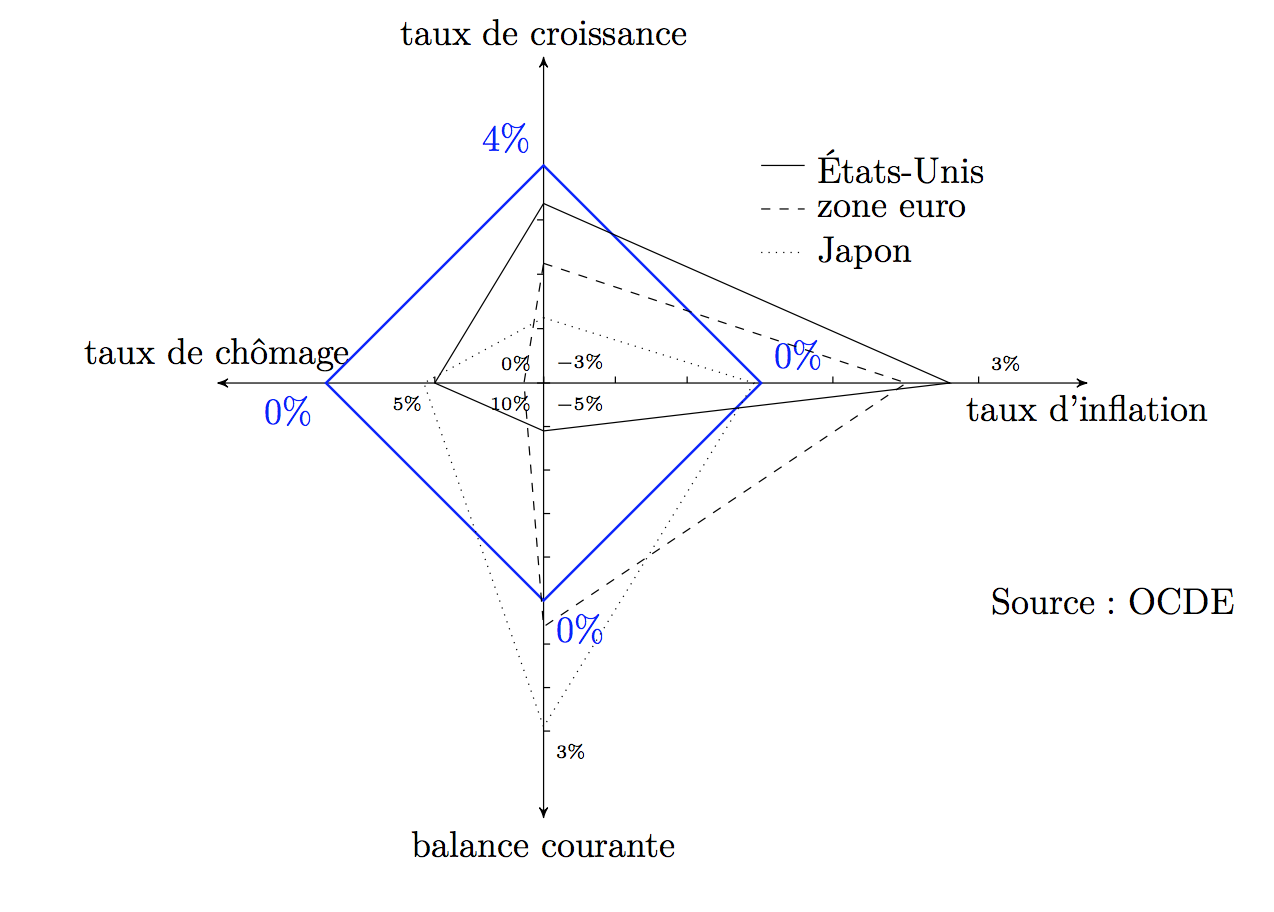
\includegraphics[scale=0.5]{./img/im2}
	\end{center}
	\caption{Carré magique : moyénné de 1996 à 2006}
  \label{fig:carre_magique}
\end{figure}

Les différents axes du \emph{carré magique} reprèsentent les objectifs de la politique macroéconomique. 
On s'intéressera dans ce chapitre aux trois premiers. 
On recueille différentes politiques économiques, chronologiquement discernables comme suit : 
\begin{itemize}[label=\ding{69}]
	\item \emph{Les trente glorieuses (45-73)} : une politique plus simple. 
  Une réponse parfaite à l'analyse keynésienne, en cas de récession et chômage élevé
	on instaurait des politques budgétaires et monétaires expansionistes (le contraire si chômage faible
  et inflation). On parle de politique de \textsc{Stop and Go}, la représentaiton économique 
  de ce phénomène s'appelle \emph{la courbe de Phillips}.
	\item \emph{À partir de soixante-dix} : on voit apparaître la \emph{stagflation}, c'est-à-dire un
  chômage croissant dans un environnement inflationniste. On retrouve pour cette période deux visions
  sur les fluctuations.
  \begin{enumerate}
    \item Selon les économistes \emph{néok-keynésiens}, l'État doit intervenir pour réguler le marché.
    \item Tandis que selon les \emph{nouveaux classiques}, l'État ne doit pas intervenir car les fluctuations
    sont des réponses naturelles du marché.
  \end{enumerate}
  \item \emph{Seconde partie des parties quatre-vingt} : la lutte contre l'inflation est le principal
  objectif des politiques. Celui-ci est atteint au moyen de politique budgétaire restrictive
  qui a entraîné des taux presque nuls et des soutiens des gouvernements moindres.
\end{itemize}

\subsection{Politique monétaire} % (fold)
\label{sub:politique_monetaire}

% subsection politique_monetaire (end)

% section conjoncture_et_politiques_economiques (end)